
% \begin{enumerate}
% \item Networking overhead 
% \item Pause-unpause overhead
% \item System overheads
% \item Effect of concurrency 
% \item Function latency vs. load 
% \item Default LB vs. Us
% \item TTL vs. GD
% \end{enumerate}

%  \vspace*{-0.2cm}
\subsection{Evaluation Environment}

\begin{figure}
  \centering
  \subfloat[Global Latency Impact]{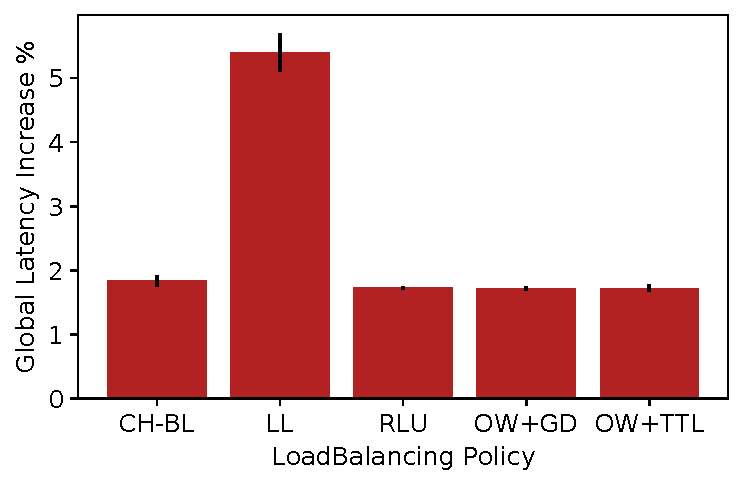
\includegraphics[width=0.5\textwidth]{chrlu/faaslb-osdi22/figs/compare/20-global-latencies-cntnorm.pdf} \label{fig:20-normalized-latencies}}
  \subfloat[Invocation Throughput]{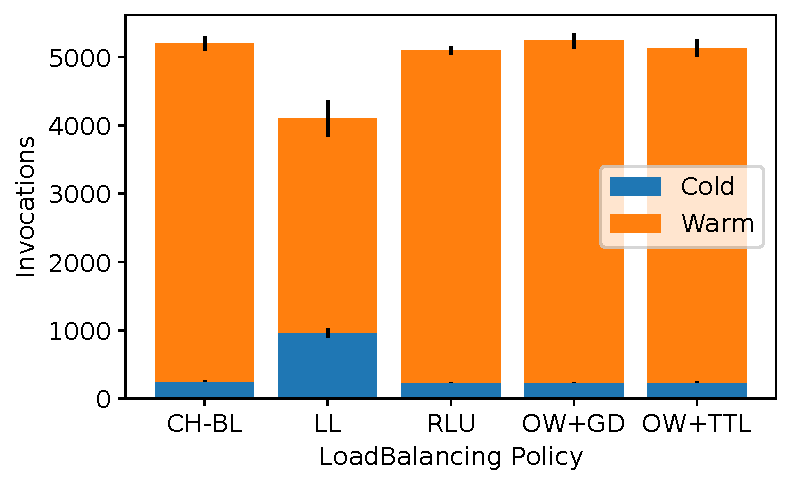
\includegraphics[width=0.5\textwidth]{chrlu/faaslb-osdi22/figs/compare/20-invokes-ttl.pdf} \label{fig:20-invokes}}
 % \vspace*{-0.5cm}
  \caption{Latency and throughput under low-load. Locality-agnostic least-loaded policy has more cold starts and a higher impact on latency.}
  \label{fig:low-load}
\end{figure}


\noindent \textbf{HW and SW Config.}
We run OpenWhisk in a distributed mode across 9 VMs.
8 invokers are each in their own VM with 16 vCPUs and assigned to use 32 GB RAM for hosting functions.
The final VM hosts the controller, load-balancer, and remaining services, with 12 vCPUs and 50 GB RAM to ensure it is not a bottleneck.
Metrics about system load were captured every 5 seconds by calling \textit{uptime} on each invokers VM and normalized by the number of CPUs on that system.
All latency information was recorded by the client, timing the HTTP request until the request completed. 
%
We make no policy changes to the invoker eviction policy, but use the changes from FaasCache~\cite{faascache-asplos21} for eviction decisions on the invoker.

\noindent \textbf{Contenders.}
In addition to our proposed load balancing policy, we compare against the default OpenWhisk load balancing policy (described in Section~\ref{subsec:ch}) with GreedyDual (OW+GD) and 10 minute Time-To-Live (OW+TTL) eviction policies, and implement two other load balancing polices for comparison: least loaded (LL), and consistent hashing with bounded loads using stale load-averages (CH-BL). 
For CH-RLU and CH-BL, we set the max\_chain\_len=3, a high max load bound, b\_max= 6, and a popularity threshold, p=20\%. 
We did not find performance to be particularly sensitive to the load-bound: the function latencies showed little changes across load upper-bounds of $[2-8]$. 
% This is also shown earlier in our latency vs. load analysis in Section~\ref{subsec:function-perf}. 

% $bounded\_ceil = 6$ because of the low correlation between a function's latency and server load from 


%%%%%%%%%%%%%%%%%%%%%%%%%%%%%%%%%%%%%%%%%%%%%%%%%%

\noindent \textbf{Metrics.}
%Evaluating the quality of a serverless load balancing policy can be done using several metrics.
We examine three main metrics: cold starts, the global average latency across all invocations, and the evenness with which load is spread amongst workers.
%
The first two directly and obviously relate to end user service quality but the third is more intricate. 
Providers pay for servers to run functions on and don't want those resources going unused and therefore wasted.
Equally, a server that is overloaded (not enough CPU or memory resources) will cause a spike in end user latency due to contention of queuing.
%
To quantify the global impact on latency from placement decisions, we normalize each invocation's latency by the ideal (minimum) latency, take the per-function mean of these, multiply each mean by the percentage of invocations that function had in the whole trace, and finally take the mean of those function latency means.
This is essentially a weighted average of latency-increase (i.e., slowdown).
It gives some balance between outcomes, for example, a rare function may get several bad placement decisions and thus increase the global latency, or a very common function generally has warm hits and does not impact latency. 
%With this metric we get a specific percentage of the increase in latency that load balancing policies have over the theoretical optimal in which all invocations have their minimum runtime.

% Setup:
% Custom OpenWhisk run on self-hosted VMs
% 8 invokers with 16 vCPUs and assignedto use 32 GB RAM for hosting functions
% Other services on 9th VM with 12 vCPUs and 50 GB RAM.


\begin{figure*}%[ht] 
  \centering
  \subfloat[Latency]{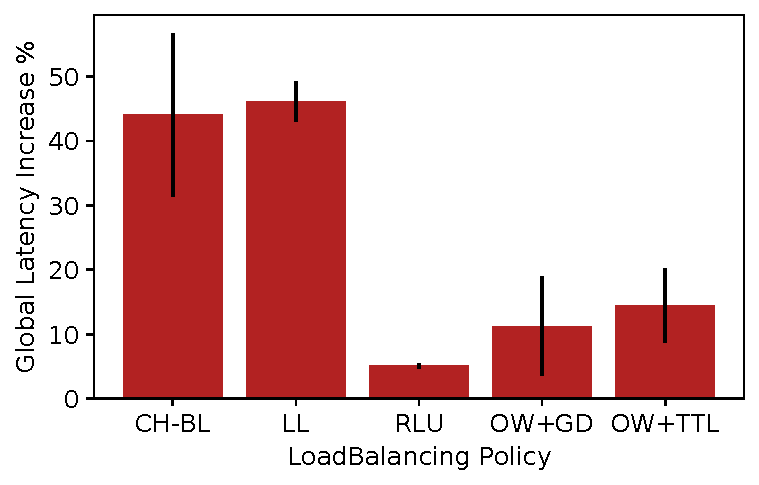
\includegraphics[width=0.4\textwidth]{chrlu/faaslb-osdi22/figs/compare/120-global-latencies-cntnorm.pdf} \label{fig:120-normalized-latencies}} 
  \hfill
  \subfloat[Throughput]{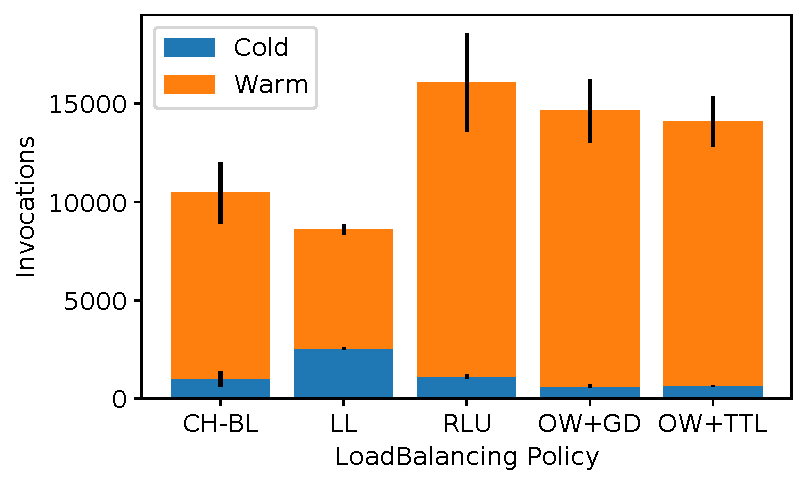
\includegraphics[width=0.4\textwidth]{chrlu/faaslb-osdi22/figs/compare/120-invokes-ttl.pdf} \label{fig:120-invokes}}
  \hfill
  \subfloat[Server Load variance]
  {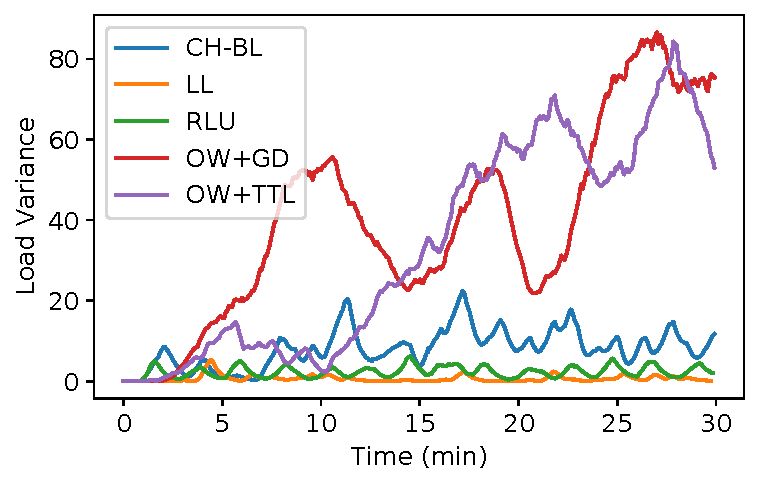
\includegraphics[width=0.4\textwidth]{chrlu/faaslb-osdi22/figs/compare/3-120-loadAvg-variance.pdf} \label{fig:120-load-variance}}
 % \vspace*{-0.5cm}
  \caption{At high server loads, our RLU policy reduces average latency by 2.2x at higher throughput, compared to OpenWhisk's default policy. It does so by keeping cold starts and load-variances low.}
  \label{fig:high-load}
\end{figure*}


\noindent \textbf{Workload.}
We convert 12 functions from FunctionBench~\cite{kim_functionbench_2019} to run on OpenWhisk.
To create a more realistic variety of functions, we create ten copies of each function with unique names, giving us 120 unique functions. 
Each function clone is invoked at different frequencies mimicking the arrival frequencies of the Azure trace~\cite{shahrad_serverless_2020}. 
% We picked these to mimic the invocation disparity shown in real-world traces.
Our load is generated using the closed-loop load generation tool Locust~\cite{locust} to invoke functions, running 20 threads for low load, and 120 for heavy load stressing.
Locust cannot easily have dedicated threads to invoke each function, so we convert the ``frequencies'' into weights and use those to randomly choose what function will be invoked next.
Each thread will iteratively invoke a random function, and after its completion wait 0-1 seconds before invoking another function.
Unless stated otherwise all experiments are run with the above settings, under heavy load, for 30 minutes, and results are the average of 4 runs.

% Workload:
% Load generated by locust
% 50 threads running in closed loop load generation (unless stated)
% 12 functions converted from FunctionBench
% mix of function types, both in runtime and resource usage
% each uploaded 4 times with unique names
% These 4 different ones will be called with diff frequencies of 1, 5, 16, 40
% mimic the invocation disparity displayed in Azure Function trace
% giving us 48 functions to call
% Load applied for 30 minutes. System stable by then and enough for a TTL impact
% each experiment run 4 times, and graphs are the average of those runs, unless stated

\begin{comment}
\subsection{Function Jitter}

\label{sec:unstable-latency}
This system added latency instability combined with the initial cold start overhead for a function's first run are two overheads no load balancing policy can mitigate.
% maybe TODO: Something on on we can only optimize warm hits and server load impact on runtime and will always have "added latency" over the optimal.

To see how our functions' latencies are affected by the system under load, we adjust the setup to have a single invoker and slowly crank up the number of threads making requests to increase the load on that invoker.
Latency increases due to load come from two causes: 1) CPU contention increases function execution time and 2) the server marshalling resources to run the function and extract results.
Figure~\ref{fig:LatencyVsLoad} shows a representative selection of functions, and the latency of individual invocations in relation to the load of our single invoker when they were invoked.
One mixed CPU and disk bound load performing web serving in Figure~\ref{fig:CHAM} sees \textit{no} impact at extreme loads.
Its only latency outliers are due to the inconsistent system overhead we saw above.
A more CPU intense function performing AES key encryption and decryption in Figure~\ref{fig:AES} roughly has some correlation with load.
Once the load gets above \textbf{8} does it not finish near its minimum latency anymore.
The AES function also exhibits layency inconsistency from the system like 'float' did, with many of the invocations under the extreme load of 10 taking as long as invocations with no load.
% Both~\ref{fig:AES} and~\ref{fig:FLOAT}, both CPU bound functions, see \textit{no} impact at extreme loads.
Finally, the long running and CPU bound Sklearn training function in Figure~\ref{fig:TRAIN} is marginally affected as load becomes extreme.
There is a definite correlation between the two, but it is clearly not linear, with a normalized load of 10 only causing a 1.5x increase in function latency.
These results challenge the traditional notion that functions are strictly limited by CPU resources. %, but we see that this isn't true.
We can favor locality more than load, allowing us to both prevent cold starts and not increase latency on warm starts.
Knowing that functions can withstand high server load up to a point, for all our following experiments we set the load bound used by RLU to 6.

\end{comment}


  %\vspace*{-0.2cm}
\subsection{Load-balancing Performance}
\label{sec:policy-comare}

% Policies being compared:
% Ours
% Bounded Loads
% Least loaded
% OpenWhisk (memory sharding) + GD
% OpenWhisk (memory sharding) + TTL

% Lots of metrics to consider when deciding a 'good' policy
% Classic cold start %
% function throughput 
% aggregated function latency
% distribution of load
%   resource usage on invokers

% The quality of a load balancing can be demonstrated in many different ways, and the addition of serverless workloads makes it more complicated.
% Our fixed-time and closed-loop load allows us to examine key metrics for FaaS and load balancing policies in general.


% global normalized latencies for 120 as a percentage over ideal
% ['CH-BL', 'LL', 'RLU', 'OW+GD', 'OW+TTL']
% [44.03687355782084, 46.12511623486831, 5.08886752197281, 11.27379780859461, 14.4173988318167]

% global normalized latencies for 20 as a percentage over ideal
% ['CH-BL', 'LL', 'RLU', 'OW+GD', 'OW+TTL']
% [1.83828219306087, 5.397093279722829, 1.7271133329324055, 1.7177648275920407, 1.723332172907966]

% Stable load
% Compare functions w/20 threads
% 20-compare-functions-ShardingContainerPoolBalancer-RLULFSharding.pdf 0.9997180360888229
% 20-compare-functions-LeastLoadBalancer-RLULFSharding.pdf 2.6262500335629335
% Compare functions w/120 threads
% 120-compare-functions-ShardingContainerPoolBalancer-RLULFSharding.pdf 1.7029922705698093
% 120-compare-functions-LeastLoadBalancer-RLULFSharding.pdf 7.805708861373892

When we run them under \textbf{light load} in Figure~\ref{fig:low-load}, the policies that use a locality mechanism are essentially identical.
The load on any one server is never high enough to impact co-located functions and we never have to forward invocations and incur excess cold starts, giving us a \quotes{lower bound} on load balancing.
The low 1-2\% latencies in Figure~\ref{fig:20-normalized-latencies} we see here are due to initial cold starts for functions and the varied overhead imparted by the system analyzed earlier.
The least loaded policy is significantly worse as it's lack of locality causes excessive cold starts as evidenced by the high number of cold starts in its invocation results detailed in Figure~\ref{fig:20-invokes}.
% The global latency impact in Figure~\ref{fig:20-normalized-latencies} and invocation throughputs in Figure~\ref{fig:20-invokes} 


Next we run the policies under our \textbf{heavy load} scenario, and get a clear distinction between how each of them performs. 
The two versions of OpenWhisk  in Figure~\ref{fig:120-normalized-latencies} only increase latency by 11\% and 14\% respectively which is rather good.
They cannot complete with RLU whos increase is less than half of that, a tiny 5\% impact on global latency.
CH-BL and least loaded increase global latency by over 40\%, showing terrible performance in that metric and on invocation throughput. 


The wide gap between policies can be understood by comparing the load variance between their workers (Figure~\ref{fig:120-load-variance}).
OpenWhisk's default policy is to only move a function to another server if the ``home'' one does not have available memory to run it. 
While very good for locality (getting fewer cold starts than RLU in Fig~\ref{fig:120-invokes}), it creates severe imbalance on the worker loads.
A few workers grow to extremely high load and their functions suffer, while others are mostly empty. 
RLU intelligently forwards invocations when a worker is near overload, keeping load variance low while protecting locality. 
Least loaded actually does the best at keeping equal load amongst workers, but at the cost of poor locality.

% An important seconday goal is to full utilize worker resources and ensure that certain workers are neither over- nor under-loaded compared to each other.
% The default OpenWhisk policy does a poor job of keeping load even on its workers, as shown in Figure~\ref{fig:OW-loadavg}
% Several workers have a load near 0, and one has a load of over 10!
% While the system has a stable mean load denoted by the solid black line, the dashed variance line is always extremely high.
% Our policy, shown in Figure~\ref{fig:Forward-loadavg} has a similar mean load to that of OpenWhisk, hovering just under 2.
% It differs by having a substantially lower variance, keeping invoker CPU load close together.
% For example invoker 4, the purple line, reaches a load of 4x at points but the system forwards work to other invokers and the load stabilizes.

%  \vspace*{-0.2cm}
\subsubsection{Handling Bursty Traffic}

% Two of the high-frequency functions have their frequency quadrupled and returned to normal every 10 seconds
% aes and gzip specifically, CPU and disk/cpu intensive respectively


\begin{figure}
  \centering
  \subfloat[Global Latency Impact]{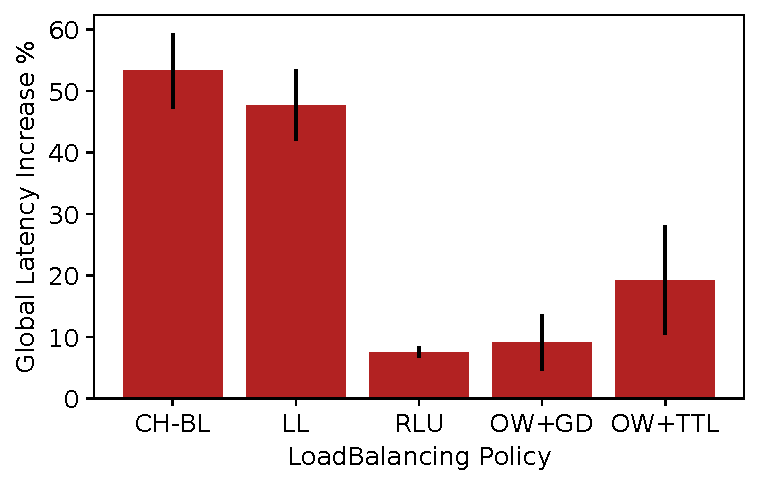
\includegraphics[width=0.5\textwidth]{chrlu/faaslb-osdi22/figs/bursty/120-global-latencies-cntnorm.pdf} \label{fig:bursty-latencies} }
  \subfloat[Worker Load Variance]{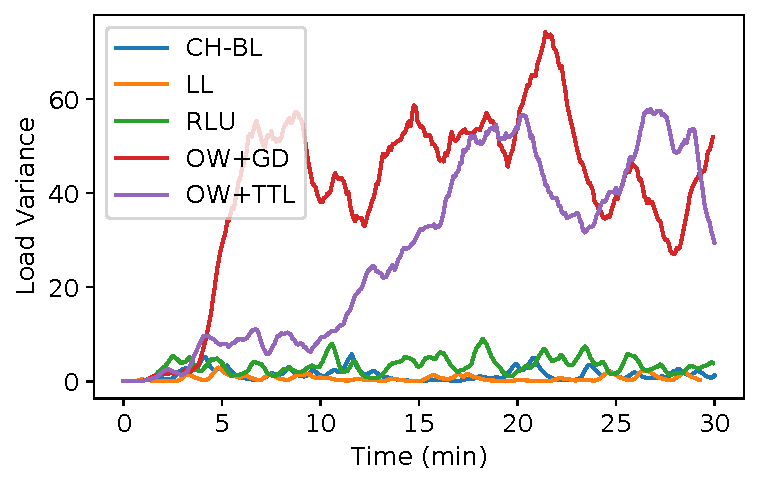
\includegraphics[width=0.5\textwidth]{chrlu/faaslb-osdi22/figs/bursty/3-120-loadAvg-variance.pdf} \label{fig:bursty-variance} }
%  \vspace*{-0.4cm}
  \caption{RLU improves latency by 10\% compared to OpenWhisk under bursty load conditions, while keeping a low worker load variance.}
  \label{fig:bursty-closedload}
\end{figure}


% Bursty load, 120 threads
% 120-compare-functions-ShardingContainerPoolBalancer-RLULFSharding.pdf 1.0932351152955206
% 120-compare-functions-LeastLoadBalancer-RLULFSharding.pdf 6.784717290259041

% global normalized latencies for 120 as a percentage over ideal
% ['CH-BL', 'LL', 'RLU', 'OW+GD', 'OW+TTL']
% [53.31502690829111, 47.720802127692316, 7.542333155555457, 9.089841768309597, 19.267038417080776]

\begin{figure}
  \centering
  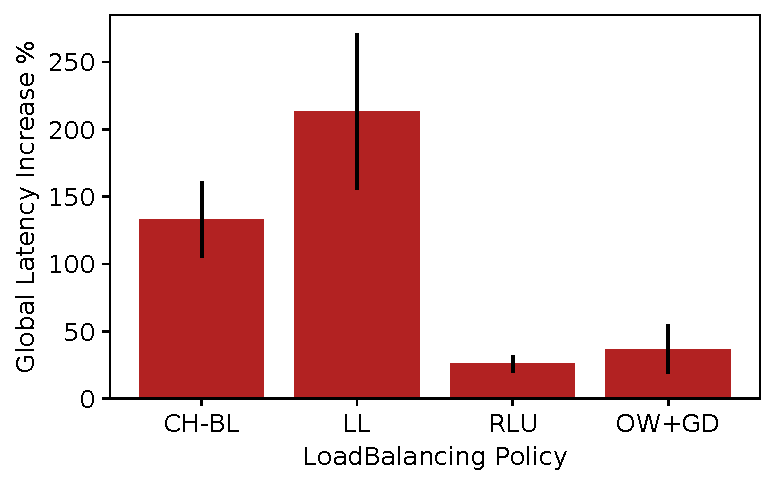
\includegraphics[width=0.6\textwidth]{chrlu/faaslb-osdi22/figs/ow/openload/openload-latencies-cntnorm.pdf}
 % \vspace*{-0.3cm}
  \caption{Global latency impact under a 30-minute long rising burst load from an open-loop generator. RLU reduces  latency by 17\% compared to OpenWhisk.}
  \label{fig:bursty-openload}
 %   \vspace*{-0.3cm}
\end{figure}

Next we take two different bursty workloads to see how the polices handle changes in invocation patterns.
The first uses the same closed-loop load generation but adjust the weights by which functions are invoked.
Every 30 seconds two of the top weighted functions are chosen to become bursty, and have their weights set much higher.
At the end of a burst their weights are returned to normal and another two functions are chosen.
As can be seen in Figure~\ref{fig:bursty-latencies} our policy acheives a 17\% lower impact on global latency than OpenWhisk with GreedyDual.
RLU represents a 60\% reduction to latency over OpenWhisk with its default TTL backend.
The more advanced eviction decision choices have a clear effect on improving the system even when the load balancer does not optimize for it.
The longer running functions in our workload have a larger effect on system load and the load balancer must be aware of this impact and either spread that heavy popular function around or move other functions off of that server.
Again, OpenWhisk does not take load into account and severely overloads some servers while languishing others.
We see more sky-high load variances from this bursty workload in Figure~\ref{fig:bursty-variance}.
Policies that monitor load, our RLU, CH-BL, and least loaded keep tighter control on load variance.

% We do suffer more cold starts, caused by moving traffic across workers to avoid load spikes from the bursty workloads.
% OpenWhisk does not try to mitigate variable workloadsd and suffers accordingly. 

% global normalized latencies for open load generation
% ['CH-BL', 'LL', 'RLU', 'OW+GD']
% [140.53344802991816, 228.83239333263217, 25.886003912929013, 36.857319393171736]

The second busrty load is a 30 minute long-rising burst, starting with just a few invocations per second and reaching a sustained peak of roughly 18 invocations per second at roughly 25 minutes.
We generated this load with a custom open-loop load tool that fires invocations but does not block waiting for completion.
New invocations are continually fired in a preset pattern of function types and times.
The global latency impact of this final scenario can be seen in Figure~\ref{fig:bursty-openload}.
Only the final 10 minutes of the workload place the system under extreme load, and the differences between policies reflect this.
CH-BL and least loaded cannot keep up with the suddenly changing load, causing a latency increase of over 100\% and 200\% respectively.
RLU's 25\% increase in global latency is still significantly better, 30\% lower, than OpenWhisk.
Our policy is able to make ideal choices for function placement under a varient of realistic workload scenarios.

\subsubsection{Scaling}
\begin{comment}
\begin{figure}
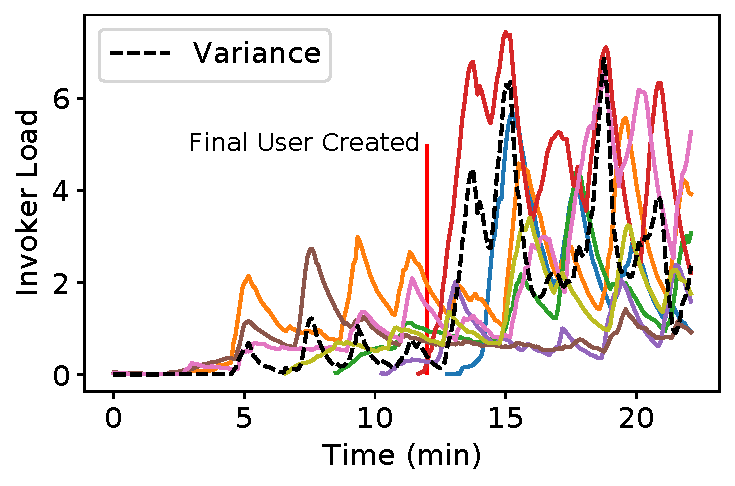
\includegraphics[width=0.33\textwidth]{../figs/scaling/120-loadAvg-6sec.pdf}
  % \vspace*{-0.3cm}
  \caption{When load increases over time, new workers are spun up and recieve a share of the workload while not being overloaded.}
  \label{fig:scaling}
%\vspace*{-0.3cm}
\end{figure}
\end{comment}

\begin{figure}  
  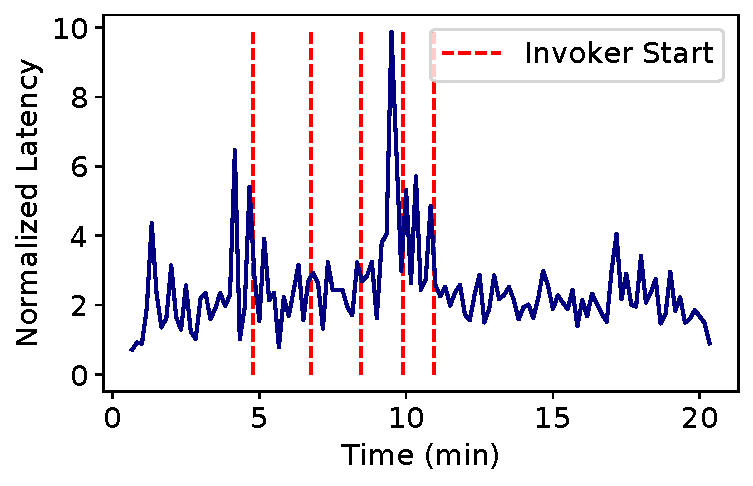
\includegraphics[width=0.6\textwidth]{chrlu/faaslb-osdi22/figs/scaling/scaling_lat_over_time-nolabel.pdf}
%  \vspace*{-0.3cm}
  \centering
  \caption{The average normalized function latency over time for a dynamic workload. New invokers are launched at the dashed lines, keeping the latency in check.}
  \label{fig:scaling-latency}
%  \vspace*{-0.3cm}
\end{figure}


% we are able to scale up infrequently and well
% system handles load as if all invokers were always up

% As described in Section~\ref{}, we can intelligently scale our systems workers as demand increases.
Lastly we want to demonstrate how our policy reacts to scaling the number of workers as demand increases.
We start our cluster with only 3 invokers and increase applied load up to the heavy load scenario above.
Rather than starting with the 120 threads of the heavy load with this smaller cluster, we adjust the scenario to start with a single thread and add a new one every 6 seconds, reaching the final thread count at about minute 12.
% Our small cluster does not allow us to match the multi-server scaling up and down changes of the simulator, so here we turn on invokers when there is an increase in forwarding to server servers beyond the 'home' server.
%The results for a single run of this scaling are in Figure~\ref{fig:scaling} with each invoker being represented by a unique color.

As the average invoker load increases, the controller activates a new worker and starts directing work towards it.
New workers are kept under the load bound of 6 and see load similar to our previous experiments that had a constant load.
%We can also correlate when new invokers are started to the latency invoked functions are encountering.
Figure~\ref{fig:scaling-latency} shows the function latencies (normalized to respective min. warm times). % and average them in 5 second groups. 
Preceeding each worker being started is a rise in overall latency, which then falls after the invoker has come online and starts taking additional load.
Thus, our horizontal scaling is able to dynamically keep the function latency in check, even though it only uses coarse-grained server load metrics.

% The remaining 5 workers are started dynamically, and quickly have a load similar to already existing workers.
% There are not load spikes or troughs, indicating the work is being spread well to new invokers as time moves on.
%These graphs are not a combination of multiple runs, but are characteristic of the performance across runs.

%\vspace*{-0.2cm}
\subsubsection{Load-balancer Overhead}

% BoundedLoadsLoadBalancer: 0.0001106853074066166
% LeastLoadBalancer: 6.170695498725195e-05
% RLULFSharding: 0.0001242685814681948
% ShardingContainerPoolBalancer: 4.7238211672012455e-05

More complicated routing decisions naturally mean they are more computationally expensive to perform.
% We have been able to keep balancing decisions to roughly 1 ms thanks to the optimizations described in Section~\ref{sec:impl}. 
Even so, RLU is on significantly slower making individual routing decisions, taking on average $1242.6 \mu$s to OpenWhisks' $472.3 \mu$s.
Such times represent a fraction of the time spent per-request by the system and is made up for by our more optimal placements. 
